\documentclass[a4paper]{article}
\usepackage{graphicx}
\usepackage{listings}
\usepackage{color}
\usepackage[hidelinks]{hyperref}

\lstset{language=Python}
\lstset{showstringspaces=false}

\title{AQA Computer Science NEA}
\author{Benjamin Lewis}
\date{2019}

\begin{document}
	\begin{titlepage}
		\maketitle
		\tableofcontents
	\end{titlepage}
	\section{Initiation}
	We were instructed to create a game that met the below criteria: 
	\begin{enumerate}
		\item 1 A menu is displayed allowing the user to select from the following options:
		\begin{itemize}
			\item Play Game
			\item Quit
		\end{itemize}
		\item If the user selects the ‘Quit’ option then a suitable message should be displayed and the program ends.
		\item If the user selects the ‘Play Game’ option they are asked to enter the number of cards to be played. If the entered number is less than 4 or greater than 30, or is an odd number, then an appropriate error message is displayed, and the user returned to the menu.
		\item The program should then read in the names of the dogs from the text file dogs.txt, creating a card for each dog.
		\item The program should randomly generate a value for each category for each dog using the ranges described on page 2, adding them to each dog’s card.
		\item The number of cards entered in task 3 are then separated into two equal piles, the player’s pile and the computer’s pile. If you wish to extend your program further then the cards may be shuffled before they are separated into two piles, however you do not have to do this.
		\item The first card in the player’s pile is displayed and the user is asked to enter a category. The categories are exercise, intelligence, friendliness and drool.
		\item The first card in the computer’s pile is then displayed.
		\item The value on the player’s card for the chosen category is compared to the value in the same category on the computer’s card.
		\begin{itemize}
			\item If the category chosen is exercise, intelligence or friendliness then the higher value wins the round.
			\item If the category chosen is drool then the lower value wins the round.
			\item If the values are the same then the player wins the round.
		\end{itemize}
		\item If the player wins the round then both cards are moved to the bottom of the player’s pile. If the computer wins the round then both cards are moved to the bottom of the computer’s pile. An appropriate message saying what the result of the comparison was and who won that round should be displayed.
		\item If the player or the computer now has all the cards then they have won the game and a suitable message should be displayed. The program should return to the main menu.
		\item Otherwise, the next round is played and the winner of the previous round chooses the category.
		\begin{itemize}
			\item If the player won the previous round then the card that is now on the top of the player’s pile is displayed and they are asked to choose a category.
			\item If the computer won the previous round then a random category is chosen. The cards that are now on the top of the player’s and computer’s piles are displayed.
			\item The game continues until the player or the computer has won.
		\end{itemize}
	\end{enumerate}
	\pagebreak
	\section{Planning}
	\paragraph{Technologies}
	I will be using python in my project as this is one of the four allowed languages by the client. Other languages I could have used are: %TODO: Insert languages here
	\subsection{Flowchart}
	\begin{center}
		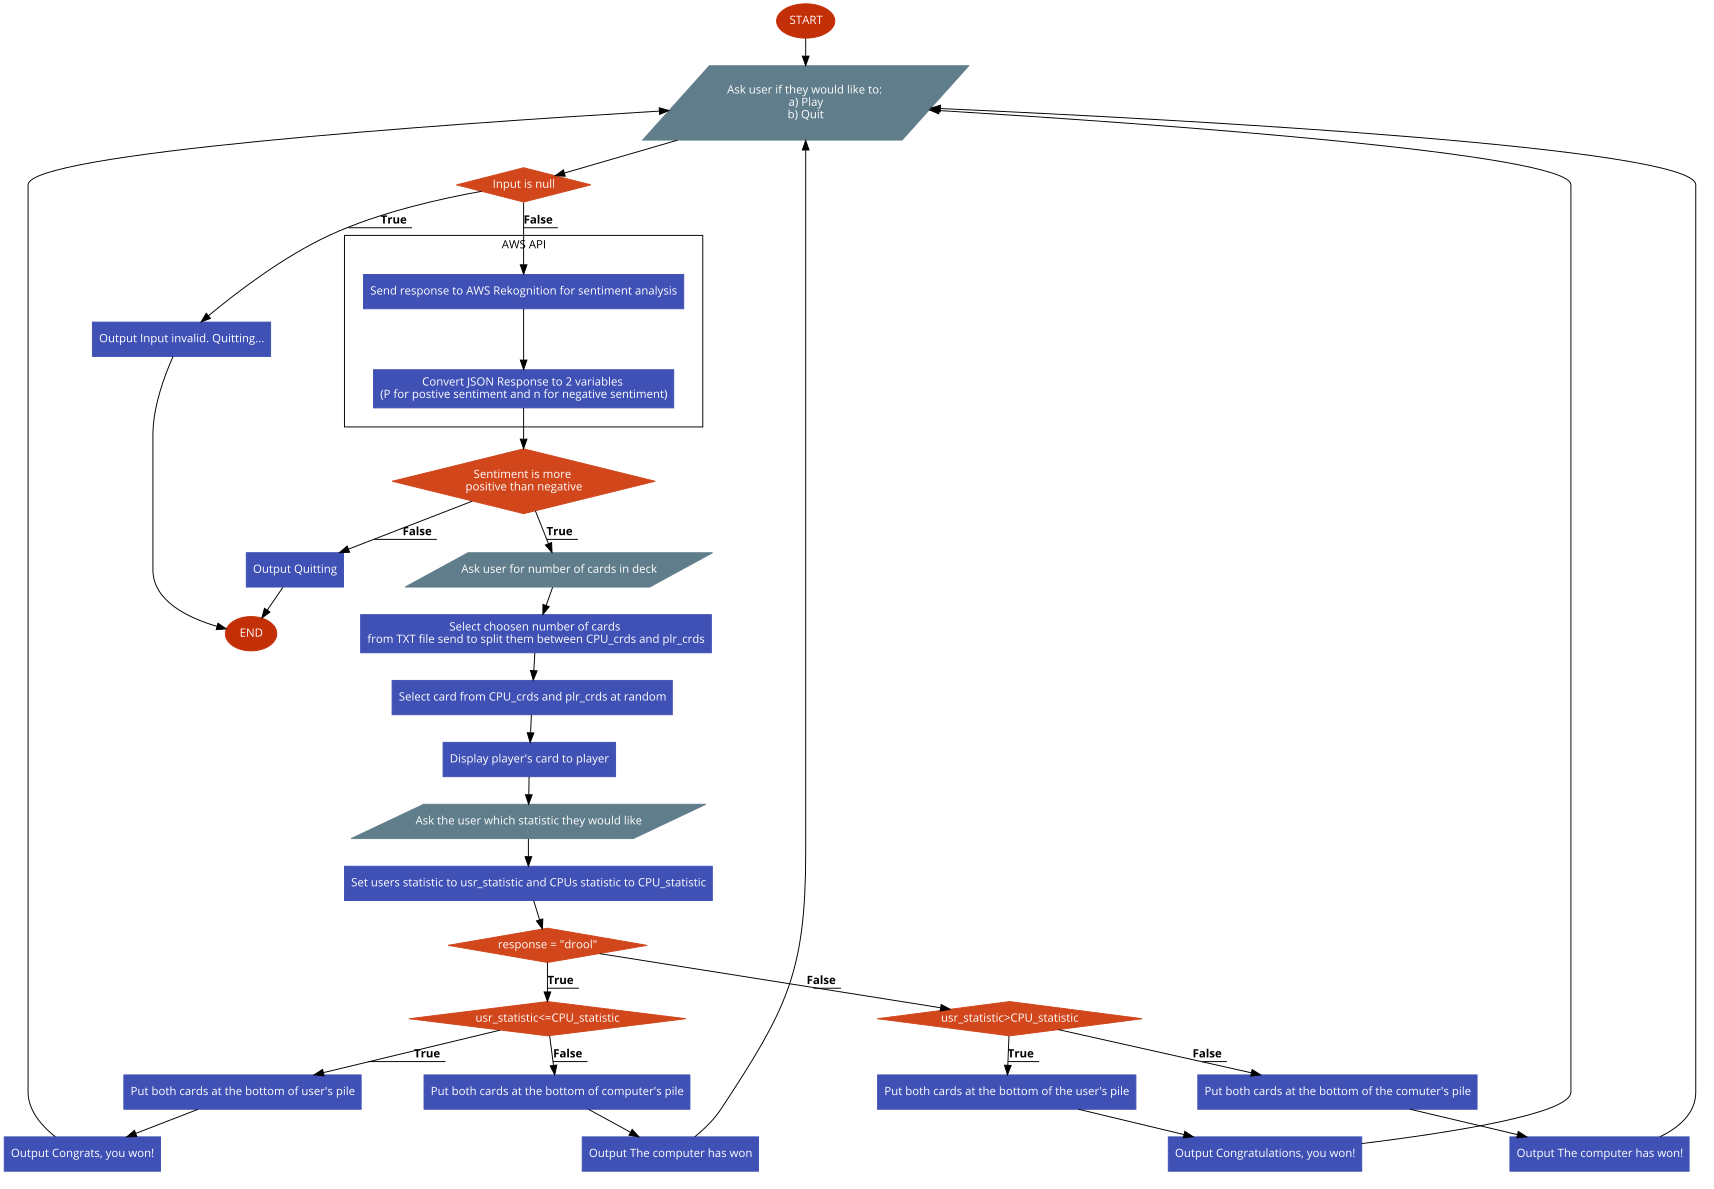
\includegraphics[width=1\linewidth]{flowchart.png}
	\end{center}
	\pagebreak
	\subsection{Pseudocode}
	\begin{lstlisting}
		START;
		before_check:
		/Ask user if they would like to: 
		a) Play
		b) Quit/;
		if (Input is null){
		Output Input invalid. Quitting...;
		return END}
		else
		block AWS API {
		Send response to AWS Rekognition for sentiment analysis;
		Convert JSON Response to 2 variables 
		(P for postive sentiment and n for negative sentiment);}
		if (Sentiment is more 
		positive than negative) {
		/Ask user for number of cards in deck/;
		Select choosen number of cards 
		from TXT file send to split them between CPU_crds and plr_crds;
		Select card from CPU_crds and plr_crds at random;
		Display player's card to player;
		/Ask the user which statistic they would like/;
		Set users statistic to usr_statistic and CPUs statistic to CPU_statistic;
		if(response = "drool"){
		if(usr_statistic<=CPU_statistic){
		Put both cards at the bottom of user's pile;
		Output Congrats, you won!;
		}else{
		Put both cards at the bottom of computer's pile;
		Output The computer has won; 
		}
		}else{
		if(usr_statistic>CPU_statistic){
		Put both cards at the bottom of the user's pile;
		Output Congratulations, you won!;
		loop before_check
		}else {
		Put both cards at the bottom of the comuter's pile;
		Output The computer has won!;
		loop before_check
		}
		};
		loop before_check;}
		else Output Quitting;
		END
	\end{lstlisting}
	\pagebreak
	\section{Development}
	\subsection{Python Code}
	\begin{lstlisting}[language=Python]
		from random import randint
		from linereader import getline
		from time import sleep
		import boto3
		import json
		
		comprehend = boto3.client(service_name='comprehend', region_name='eu-west-1')
		
		while 1: 
		choice = str.lower(input("What would you like to do? (Play/ Quit)"))
		if choice != "":
			result = comprehend.detect_sentiment(Text=choice, LanguageCode='en') #, sort_keys=True, indent=4)
			p = result["SentimentScore"]["Positive"]
		else: 
			print("No input detected, quitting...")
			sleep(1)
			break
		if p>=n:
			dname = getline("dogs.txt", randint(1,30))
			excersise = randint(1,5)
			inteligence = randint(1,100)
			friendliness = randint(1,10)
			drool = randint(1,10)
			print("Welcome!")
			print("Excersise: ", excersise)
			print("Intelignece: ", inteligence)
			print("Friendliness: ", friendliness)
			print("Drool: ", drool)
			print(dname)
			selection = input("Please select a category... \n")
			if selection.lower() == "drool":
				print("You selected drool")
			else: 
				print("You did not select drool")
		else:
			print("Exiting...")
			break
	\end{lstlisting}
	\subsection{Version Control}
	In order to maintain different versions of the file and ensure that files can be recovered in the case of an issue with the data, I utilised the git version control standard and a repository hosted on GitHub. The repository can be found at: \url{https://github.com/benjisoft/Dog-NEA}
	\pagebreak
	\section{Evaluation}
	\subsection{Testing}
	When tested, all of the completed code works as intended. However, the code is incomplete at time of publishing. Due to this, the project does not work to the client requirements. 
	\subsection{Conclusion}
	In order to improve, the code should be finished and in future, I will put contingency plans into place in order to prevent projects from not being completed to the specified deadline. 
\end{document}